\chapter[Polynomial chaos and sparse regression]{Polynomial chaos, sparse regression and response surfaces}
\label{ch:pce}

Chapter~\ref{ch:gp} chose a kernel and let the basis be infinite. This chapter goes the other way: choose a finite
basis of polynomials, believe that only a few of its terms matter, and fit their coefficients. Done with the right
polynomials this is \emph{polynomial chaos} (PCE), the workhorse of uncertainty quantification; done with a full
quadratic it is the engineer's \emph{response surface}. Both are least squares (Section~\ref{sec:ls}) with a
well-chosen basis, plus one new idea that carries most of the weight in high dimension: \emph{sparsity}.

\section{From one input to many}
\label{sec:pce_basis}

In one variable on $[-1,1]$, Chapter~\ref{ch:toolkit} built the Legendre polynomials by Gram--Schmidt and saw that
they fix the conditioning problem of monomials. We use them \emph{orthonormal} under the uniform probability measure
$dx/2$: $\psi_k(x) = \sqrt{2k+1}\,P_k(x)$, so that $\E[\psi_j\psi_k] = \tfrac12\int_{-1}^1 \psi_j\psi_k\,dx =
\delta_{jk}$.

In $d$ variables, take products. A \emph{multi-index} $\alpha = (\alpha_1,\dots,\alpha_d) \in \mathbb{N}^d$ names
the polynomial
\begin{equation}
  \Psi_\alpha(x) = \prod_{j=1}^d \psi_{\alpha_j}(x_j), \qquad \E[\Psi_\alpha\Psi_\beta] = \prod_j
  \E[\psi_{\alpha_j}\psi_{\beta_j}] = \delta_{\alpha\beta},
  \label{eq:tensor_basis}
\end{equation}
where the expectation factorises because the inputs are independent. Orthonormality in one variable gives it in $d$
for free. The surrogate is $\hat f(x) = \sum_{\alpha \in \mathcal{A}} c_\alpha \Psi_\alpha(x)$ for some finite set
$\mathcal{A}$ of multi-indices.

\paragraph{Which multi-indices?} The \emph{total-degree} set $\{\alpha : \sum_j \alpha_j \le p\}$ keeps every
polynomial of degree at most $p$. Its size is
\begin{equation}
  P = \binom{d+p}{p} \;\approx\; \frac{d^{\,p}}{p!} \quad (d \gg p),
\end{equation}
polynomial in $d$ rather than exponential, but still large. The \emph{hyperbolic} set $\{\alpha : \norm{\alpha}_q \le
p\}$ with $0 < q < 1$ keeps all the pure powers $x_j^{p}$ and cuts high-order interactions such as $x_1x_2x_3x_4x_5$:
\begin{center}
\small
\begin{tabular}{rrrrrrrrrr}
\toprule
 & \multicolumn{3}{c}{$p = 2$} & \multicolumn{3}{c}{$p = 3$} & \multicolumn{3}{c}{$p = 5$} \\
\cmidrule(lr){2-4}\cmidrule(lr){5-7}\cmidrule(lr){8-10}
$d$ & total & $q{=}0.75$ & $q{=}0.5$ & total & $q{=}0.75$ & $q{=}0.5$ & total & $q{=}0.75$ & $q{=}0.5$ \\
\midrule
2  & 6   & 5  & 5  & 10    & 8   & 7  & 21     & 16    & 12  \\
5  & 21  & 11 & 11 & 56    & 26  & 16 & 252    & 86    & 36  \\
10 & 66  & 21 & 21 & 286   & 76  & 31 & 3\,003 & 396   & 96  \\
20 & 231 & 41 & 41 & 1\,771 & 251 & 61 & 53\,130 & 2\,191 & 291 \\
\bottomrule
\end{tabular}
\end{center}
The study's \texttt{pce\_lars} uses $q = 0.75$ and chooses $p$ from $n$ and $d$, lowering it until the basis has at
most 2\,000 terms.

\begin{intuition}[Why cutting interactions is usually safe]
Most engineering responses are dominated by main effects and low-order interactions: the \emph{sparsity-of-effects}
principle of experimental design. A term like $x_1x_2x_3x_4x_5$ says ``the effect of $x_1$ depends on the
values of four other inputs at once''; such effects exist, but they are rarely large. The hyperbolic set bets on
this, the same way Chapter~\ref{ch:toolkit}'s curse of dimensionality says every surrogate must bet on some
structure.
\end{intuition}

\section{Polynomial chaos: orthogonal under the input distribution}
\label{sec:chaos}

In uncertainty quantification the inputs are random, $X \sim \rho$, and so is the output $Y = f(X)$. A
\emph{polynomial chaos expansion} writes $Y$ in polynomials that are orthonormal under $\rho$:
\begin{equation}
  Y = f(X) = \sum_{\alpha} c_\alpha \Psi_\alpha(X), \qquad c_\alpha = \E[f(X)\,\Psi_\alpha(X)] = \int f\,\Psi_\alpha\,
  \rho\,dx .
  \label{eq:pce}
\end{equation}
The coefficient formula is projection (Result~\ref{res:projection}) in the inner product $\ip{g}{h} = \E[g(X)h(X)]$,
the $L^2(\rho)$ space of finite-variance functions of the inputs. Each input distribution has its own family
(the \emph{Wiener--Askey scheme}, Xiu and Karniadakis):
\begin{center}
\small
\begin{tabular}{p{3.4cm}p{2.0cm}p{8.2cm}}
\toprule
input distribution & polynomials & where they appear \\
\midrule
uniform on an interval & Legendre & bounded design variables; every learner in the study (inputs mapped to $[0,1]^d$) \\
Gaussian & Hermite & Wiener's original ``homogeneous chaos'' (1938) \\
gamma & Laguerre & positive quantities with a long tail \\
beta & Jacobi & bounded but non-uniform inputs \\
\bottomrule
\end{tabular}
\end{center}
For Gaussian inputs, the Cameron--Martin theorem guarantees that the Hermite expansion converges in mean square for
\emph{every} finite-variance $f$; for the other families the corresponding statement needs the distribution to be
determined by its moments, which holds for all the bounded ones above. Inputs with another distribution are first
mapped to one of these (an \emph{isoprobabilistic transform}); dependent inputs need a transform that removes the
dependence (Rosenblatt, Nataf), a point we return to under sensitivity.

\begin{connection}[Chaos in the random space, POD in the physical space]
Chapter~\ref{ch:gp}'s Karhunen--Lo\`eve expansion writes a random \emph{field} as $\sum_j \sqrt{\lambda_j}\,\xi_j\,
\psi_j(x)$: deterministic modes in physical space, random amplitudes. Polynomial chaos expands the random amplitudes
themselves as polynomials of the underlying inputs. Stochastic finite elements (Ghanem and Spanos) combine the two,
KL for the random field in space and PCE for how the solution depends on the KL variables. Substituting the
expansion into the governing equations and projecting with a Galerkin condition gives \emph{intrusive} (stochastic
Galerkin) PCE, the stochastic cousin of a Galerkin reduced-order model; fitting the coefficients from solver runs,
as here, is \emph{non-intrusive}. The study is entirely non-intrusive.
\end{connection}

\begin{pitfall}
``Chaos'' here has nothing to do with chaotic dynamics; it is Wiener's 1938 word for a random process. And a PCE is
a surrogate like any other: nothing about it is specific to probability until you read statistics off its
coefficients (Section~\ref{sec:sobol}).
\end{pitfall}

\section{How fast the coefficients fall}
\label{sec:decay}

Truncating \eqref{eq:pce} after a set $\mathcal{A}$ leaves an error whose mean square is the sum of the squared
coefficients left out, $\E[(f - \hat f)^2] = \sum_{\alpha \notin \mathcal{A}} c_\alpha^2$ (Pythagoras in an
orthonormal basis). So everything depends on how fast $|c_\alpha|$ falls. In one variable the answer is classical,
and it is the $s$ of Chapter~\ref{ch:toolkit}'s rate in a sharper form.

\begin{result}[Smoothness decides the decay]
\label{res:decay}
For Legendre coefficients on $[-1,1]$:
\begin{enumerate}[nosep]
  \item If $f$ is analytic inside the \emph{Bernstein ellipse} with foci $\pm1$ and semi-axis sum $\rho > 1$, then
        $|c_k| \le C \rho^{-k}$: geometric decay, faster the further the nearest singularity is from $[-1,1]$.
  \item If $f$ has $s$ derivatives with the $s$-th of bounded variation, the decay is algebraic, roughly
        $|c_k| \lesssim k^{-(s+1)}$ in the orthonormal normalisation.
\end{enumerate}
\end{result}
\begin{intuition}
Substitute $x = \cos\theta$: a Legendre series in $x$ behaves like a Fourier series in $\theta$, and Fourier
coefficients fall exponentially for functions analytic in a strip and algebraically for functions with finitely
many derivatives (each integration by parts gains a factor $1/k$ until a derivative stops being smooth). The
Bernstein ellipse is the image of that strip under $\cos$. A singularity in the complex plane, even one you never
see on the real line, sets the size of the ellipse.
\end{intuition}

Figure~\ref{fig:decay} checks this numerically. $e^{x}$ is entire: its coefficients reach the round-off floor
($10^{-12}$) by degree 12. Runge's function $1/(1+25x^2)$ is analytic on $[-1,1]$ but has poles at $\pm i/5$, which
gives $\rho = 1/5 + \sqrt{1 + 1/25} = 1.2198$; the measured coefficients fall by a factor $0.820$ per degree against
the predicted $1/\rho = 0.8198$. The kink $|x|$ ($s = 1$) gives a fitted power $-1.97$ and the jump
$\operatorname{sign}(x)$ ($s = 0$) gives $-0.98$, matching $k^{-(s+1)}$. A jump therefore needs about ten times as
many terms for each extra digit of accuracy as a kink, and polynomial surrogates of discontinuous responses are
slow and ring near the jump (the Gibbs phenomenon).

\begin{figure}[t]
  \centering
  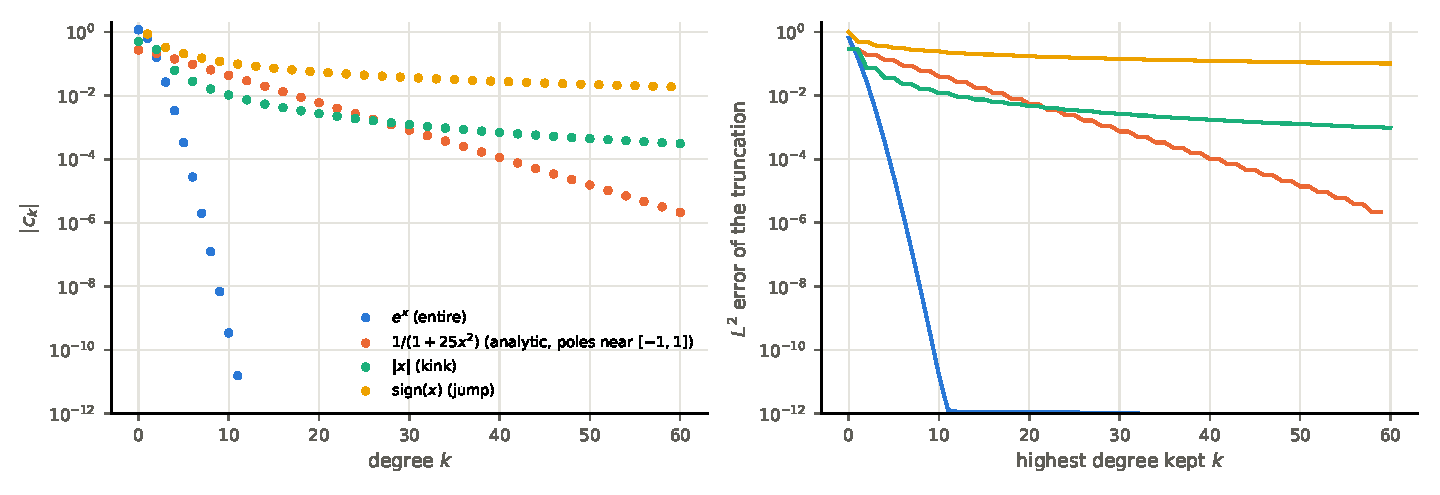
\includegraphics[width=\textwidth]{figures/ch03_coeff_decay.pdf}
  \caption{Left: orthonormal Legendre coefficients of four functions on $[-1,1]$ (zeros from symmetry omitted).
  Right: $L^2$ error of keeping the first $k+1$ terms. Analytic functions converge geometrically, a kink like
  $k^{-2}$, a jump like $k^{-1}$.}
  \label{fig:decay}
\end{figure}

\begin{pitfall}[Runge is about the points, not the polynomials]
Runge's function is famous for interpolation at \emph{equally spaced} points diverging as the degree grows. That is a
failure of the sample points, not of polynomials: the best polynomial approximation converges geometrically, as the
figure shows, and interpolation at Chebyshev points (which cluster at the ends) converges too. Least squares on
random or Sobol' points sits in between and is safe when the number of samples comfortably exceeds the number of
terms (next section).
\end{pitfall}

\section{Computing the coefficients}

\paragraph{By projection (quadrature).} Approximate $c_\alpha = \E[f\Psi_\alpha]$ with a quadrature rule.
Gauss--Legendre with $m$ nodes integrates every polynomial of degree up to $2m-1$ exactly, so with $m = p+1$ nodes
per axis the coefficients of a degree-$p$ polynomial $f$ are exact. In $d$ dimensions a tensor rule needs $m^d$
evaluations, which is the full grid of Chapter~\ref{ch:toolkit}'s curse. Smolyak's \emph{sparse grids} combine
low-order tensor rules with signed weights so that only the low-total-degree part is integrated exactly, at a cost
that grows like $m(\log m)^{d-1}$ instead of $m^d$; the study's self-designing Smolyak surrogate (E14) and
sparse-grid upscaler (E8) are this construction. Quadrature needs $f$ at the nodes it chooses, so it suits a solver
you can run on demand, not a given data set.

\paragraph{By regression.} With samples $x_1,\dots,x_n$ and the design matrix $\Phi_{i\alpha} = \Psi_\alpha(x_i)$,
solve least squares $\min_c \norm{\Phi c - y}^2$ by QR or SVD (Section~\ref{sec:ls}). Orthonormality of the basis
under $\rho$ means $\tfrac1n\Phi\T\Phi \to I$ as $n$ grows with samples drawn from $\rho$, so the problem becomes
perfectly conditioned in the limit; Chapter~\ref{ch:toolkit}'s monomial disaster does not arise. How many samples are
enough for $\tfrac1n\Phi\T\Phi$ to be \emph{close} to $I$ depends on how large the basis functions get: the high-degree
Legendre polynomials are largest at the ends of the interval, and with uniform samples the safe number grows faster
than linearly in the number of terms $P$. Sampling more densely near the boundary (Chebyshev-like, or the ``optimal''
Christoffel-weighted density of Cohen and Migliorati) brings it down to about $P\log P$. The usual rule of thumb is
$n \approx 2$--$3P$ samples for plain least squares.

\begin{pitfall}[More terms than samples]
In high dimension the rule of thumb fails immediately: $d = 10$, $p = 3$ already has $P = 286$ terms, while the
study's designs have $n = 10d$ to $100d$ points. With $n < P$ least squares has infinitely many exact fits, and the
minimum-norm one (what \texttt{lstsq} returns) spreads energy over all terms. The next section is the way out.
\end{pitfall}

\section{Sparsity: the LASSO and least-angle regression}
\label{sec:sparse}

If only $s \ll P$ coefficients matter, the problem is not $P$ unknowns but $s$ unknowns at unknown positions. The
convex way to look for them replaces ridge's squared penalty with an absolute-value one, the \emph{LASSO}
(Tibshirani):
\begin{equation}
  \hat c = \argmin_c \; \tfrac12\norm{y - \Phi c}^2 + \lambda \norm{c}_1, \qquad \norm{c}_1 = \sum_\alpha |c_\alpha| .
  \label{eq:lasso}
\end{equation}

\begin{result}[In an orthonormal design the LASSO soft-thresholds]
\label{res:soft}
If $\Phi\T\Phi = I$ and $b = \Phi\T y$ is the least-squares solution, then
$\hat c_\alpha = \operatorname{sign}(b_\alpha)\max(|b_\alpha| - \lambda, 0)$. Ridge, by contrast, gives
$b_\alpha/(1+\lambda)$.
\end{result}
\begin{intuition}
With $\Phi\T\Phi = I$ the objective separates into one problem per coefficient,
$\tfrac12(c - b)^2 + \lambda|c|$. Away from $0$ its derivative is $c - b \pm \lambda$, so the minimiser is $b$
moved towards zero by $\lambda$; if $|b| \le \lambda$ the kink of $|c|$ at zero wins and the minimiser is exactly
$0$. Ridge only shrinks by a factor and never reaches zero (Chapter~\ref{ch:toolkit}'s filter factors), so it never
selects. Geometrically: the $\ell_1$ ball is a diamond whose corners lie on the axes, and the first point of the
diamond that a growing ellipse of least-squares contours touches is usually a corner, where most coordinates are zero.
\end{intuition}

\paragraph{Least-angle regression (LARS).} The LASSO solution changes piecewise linearly as $\lambda$ decreases from
``everything zero'' to ``least squares'', and LARS (Efron, Hastie, Johnstone and Tibshirani) traces this whole
\emph{path} for about the cost of one least-squares fit:
\begin{enumerate}[nosep]
  \item Start with $c = 0$ and residual $r = y$. Find the basis function most correlated with $r$.
  \item Move its coefficient towards its least-squares value until a second basis function is equally correlated
        with the residual.
  \item Then move both together, along the direction that keeps their correlations equal (the ``least angle'',
        equiangular, direction), until a third joins; and so on.
  \item (LASSO modification) if a coefficient would cross zero, drop it from the active set.
\end{enumerate}
Each step adds one term, so the path is a sequence of increasingly rich sparse models. Which point on the path to
keep is decided by cross-validation (Section~\ref{sec:measure}). The study's \texttt{pce\_lars} does exactly this
(scikit-learn's \texttt{LassoLarsCV}, 5 folds) on the hyperbolic Legendre basis. The UQ literature's version (Blatman
and Sudret) refits each candidate support by ordinary least squares and chooses by leave-one-out error, which
removes the LASSO's shrinkage of the kept coefficients; the study keeps the plain LASSO estimate.

\begin{result}[Compressed sensing, informally]
If $f$ is exactly $s$-sparse in a bounded orthonormal basis of $P$ functions, and the $n$ samples are drawn at
random from the right measure, then with high probability $\ell_1$ minimisation recovers the coefficients exactly
once $n$ is of order $s$ times powers of $\log P$, far fewer than $P$ (Cand\`es, Romberg and Tao; Donoho; Rauhut
and Ward for orthogonal polynomials). With noise or approximate sparsity the error is close to the best $s$-term
approximation.
\end{result}
\begin{intuition}
A random sampling matrix acts almost like an isometry on every sparse vector at once (the restricted isometry
property): no two sparse coefficient vectors produce nearly the same samples, so the samples pin down the sparse
vector, and $\ell_1$ is the convex relaxation that finds it. The price of not knowing \emph{where} the $s$ terms
are is only logarithmic.
\end{intuition}

Figure~\ref{fig:sparse} puts numbers on it. A function of $d = 10$ inputs with 8 nonzero coefficients in the
total-degree-3 basis ($P = 286$), sampled on Sobol' points with 1\% noise:
\begin{center}
\small
\begin{tabular}{rccccl}
\toprule
$n$ & least squares & ridge (CV) & LASSO--LARS (CV) & terms kept & true terms found \\
\midrule
30  & 1.03  & 1.05  & 0.94  & 11 & 2 of 7 \\
60  & 0.91  & 0.94  & 0.004 & 40 & 7 of 7 \\
120 & 0.86  & 0.86  & 0.003 & 31 & 7 of 7 \\
240 & 0.40  & 0.40  & 0.001 & 27 & 7 of 7 \\
480 & 0.005 & 0.005 & 0.001 & 25 & 7 of 7 \\
\bottomrule
\end{tabular}
\end{center}
(test NRMSE). From $n = 60$, about a fifth of $P$, the LASSO is essentially exact while least squares and ridge
are no better than predicting the mean; they catch up only once $n > P$. Below about 60 points recovery fails
abruptly, the phase transition that compressed-sensing theory predicts. Note the kept terms: the LASSO also keeps
20 to 30 tiny spurious coefficients. They cost little accuracy here, but they are why a refit by least squares on
the selected support, or a sharper criterion than plain cross-validation, is common in practice.

\begin{figure}[t]
  \centering
  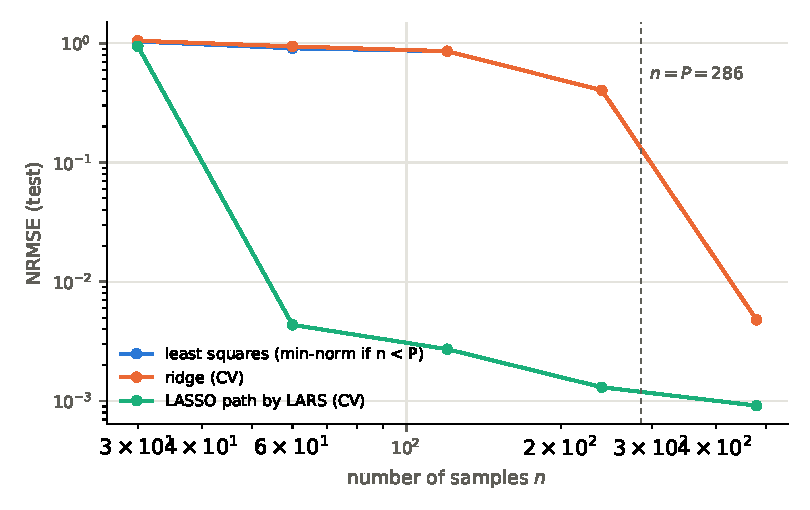
\includegraphics[width=0.62\textwidth]{figures/ch03_sparse.pdf}
  \caption{Test error against the number of samples for an 8-term function of 10 inputs in a 286-term basis. The
  sparse fit needs about a fifth as many samples as the basis has terms; least squares and ridge need more samples
  than terms.}
  \label{fig:sparse}
\end{figure}

\begin{connection}[SINDy: sparse regression for dynamics]
Sparse identification of nonlinear dynamics (Brunton, Proctor and Kutz) applies the same idea to $\dot x = g(x)$:
build a library of candidate terms (polynomials in the state, trigonometric functions), regress measured time
derivatives on it with a sparsity-promoting method, and read off the few terms that remain as the governing
equation. Where DMD fits the best \emph{linear} operator, SINDy fits the sparsest \emph{nonlinear} one in a chosen
library. Both live or die by the same assumption as sparse PCE: the right basis makes the answer short.
\end{connection}

\section{Statistics for free: mean, variance and Sobol' indices}
\label{sec:sobol}

Because the basis is orthonormal under the input distribution and $\Psi_0 = 1$, the moments of the surrogate are read
off its coefficients without any further sampling:
\begin{equation}
  \E[\hat f] = c_0, \qquad \Var[\hat f] = \sum_{\alpha \ne 0} c_\alpha^2 .
\end{equation}

\paragraph{Variance-based sensitivity.} Sobol' decomposes $f$ into a constant, functions of one input, functions of
two, and so on, $f = f_0 + \sum_i f_i(x_i) + \sum_{i<j} f_{ij}(x_i,x_j) + \cdots$ (the ANOVA decomposition), with
every term of zero mean in each of its own variables. The pieces are orthogonal, so the variance splits too, and the
\emph{first-order index} $S_i = \Var[f_i]/\Var[f]$ is the share of the variance due to $x_i$ alone; the \emph{total
index} $S_{T_i}$ adds every interaction that involves $x_i$.

\begin{result}[Sobol' indices from a PCE (Sudret)]
Group the terms by which inputs they involve. Then
\begin{equation}
  S_i = \frac{\sum_{\alpha \in \mathcal{A}_i} c_\alpha^2}{\sum_{\alpha \ne 0} c_\alpha^2},\quad
  \mathcal{A}_i = \{\alpha: \alpha_i > 0,\ \alpha_j = 0 \ (j \ne i)\};\qquad
  S_{T_i} = \frac{\sum_{\alpha:\, \alpha_i > 0} c_\alpha^2}{\sum_{\alpha \ne 0} c_\alpha^2}.
\end{equation}
\end{result}
\begin{intuition}
A product polynomial $\Psi_\alpha$ depends on exactly the inputs with $\alpha_j > 0$ and has zero mean in each of
them, so grouping the PCE terms by their support \emph{is} the ANOVA decomposition. Parseval then turns each
piece's variance into a sum of squared coefficients.
\end{intuition}

On the Ishigami function, $f = \sin x_1 + 7\sin^2 x_2 + 0.1\,x_3^4\sin x_1$ on $[-\pi,\pi]^3$, a standard test with
exact answers ($S_1 = 0.3139$, $S_2 = 0.4424$, $S_3 = 0$, $S_{T_3} = 0.2437$): a sparse PCE of total degree 14 fitted
by LASSO--LARS to 100 Sobol' points gives $0.3140$, $0.4427$, $0.0000$ and $0.2433$, and from 200 points all six
indices agree to four decimals. The standard Monte Carlo (pick-freeze) estimator, which needs $N(d+2)$ runs, gives
$S_1, S_2 = 0.269, 0.383$ from 5\,000 runs and $0.322, 0.436$ from 50\,000. When the PCE fits, it is a thousand times
cheaper.

\begin{pitfall}
The formulas assume independent inputs with the distribution the basis is orthonormal for. With dependent inputs
the ANOVA terms are no longer orthogonal and ``the share of variance due to $x_i$'' is not uniquely defined. And the
indices are those of the surrogate: a poorly fitted PCE gives confident, wrong sensitivities.
\end{pitfall}

\section{The quadratic response surface}
\label{sec:rsm}

The oldest polynomial surrogate is the full quadratic,
$\hat f(x) = \beta_0 + \sum_i \beta_i x_i + \sum_{i \le j} \beta_{ij}x_ix_j$, with $(d+1)(d+2)/2$ coefficients: the
total-degree-2 basis written in monomials. Box and Wilson introduced it (1951) to find optimal operating conditions
of chemical processes by fitting a quadratic around the current best point and moving to its stationary point, and
designs such as the central composite design were built to estimate exactly these coefficients. The study's
\texttt{rsm2} fits it by least squares with a tiny ridge for stability.

A quadratic cannot bend twice, so as a global approximation of a multimodal function it is poor. Yet it is a
surprisingly good surrogate \emph{for optimization}. In E9, \texttt{rsm2} had a median NRMSE of 0.45, among the
least accurate surrogates tested, but reached the true optimum (regret below 1\% of the spread of $f$) in 41\% of
tasks with its best optimizer, about as often as the sparse PCE and twice as often as CatBoost or LightGBM, which are
more accurate (NRMSE 0.34--0.35) but piecewise constant.

\begin{intuition}
An optimizer needs the surrogate's minimiser to lie near the true one, not its values to be right. A least-squares
quadratic captures the large-scale trend of the data, it is smooth and has a single stationary point, and every
optimizer finds that point. When the true function has a dominant basin, the quadratic's minimum lands in it. This
is Chapter~\ref{ch:toolkit}'s distinction between accuracy and decision quality in its simplest form, and the
reason trust-region methods for expensive problems (Powell's derivative-free solvers, the model-management loops of
the study's E9b) build \emph{local} quadratics: near a minimum, every smooth function looks like one.
\end{intuition}

\section{When polynomials are the wrong model}

\begin{center}
\small
\begin{tabular}{p{4.1cm}p{5.3cm}p{4.2cm}}
\toprule
Property of $f$ & Why a global polynomial struggles & Remedy (later chapters) \\
\midrule
Jumps, kinks, plateaus & algebraic coefficient decay (Result~\ref{res:decay}); Gibbs ringing & multi-element PCE,
trees, partitioned models \\
Singularity near the domain (a pole, a knee) & small Bernstein ellipse: slow geometric decay & rational
approximation \\
Many inputs that all interact & $P$ explodes and $f$ is not sparse in the basis & low-rank and tensor-train models \\
Local features (a narrow bump) & a bump needs many global terms & kernels and RBF (Chapter~\ref{ch:gp}) \\
Predicting outside the sampled box & polynomials grow like $|x|^p$ off the data & stay inside the box; bound the
optimizer \\
Dependent or unusual input distributions & orthogonality and Sobol' formulas assume independence & transforms
(Rosenblatt, Nataf), data-driven arbitrary PCE \\
\bottomrule
\end{tabular}
\end{center}

\paragraph{What the study found.} On the 80 problems of the original E3 set, \texttt{pce\_lars} ranked tenth of 38
methods (geometric-mean error $2.45\times$ the per-cell best); on the 89 problems added in E3x, which include many
smooth classical benchmark functions, it ranked first ($1.71\times$), a difference significant after Holm correction
($p = 0.0006$). Across all 169 problems it was the method with the best average rank, while the agreement between
problems on the ranking was weak (Kendall's $W = 0.37$): the best \emph{single} choice, and still a long way from the
best choice for each problem. It lost to trees on the rugged, discontinuous problem type, as the table predicts.

\section*{Notes}
\begin{itemize}[leftmargin=*,nosep]
  \item Derivatives of a PCE are polynomials again, available in closed form; the study's gradient study (E13)
        includes a gradient-enhanced PCE that adds $\partial f/\partial x_j$ samples as extra rows of $\Phi$.
  \item Orthogonal matching pursuit is a greedy alternative to the LASSO (add the most correlated term, refit by least
        squares, repeat); the study's compressed-sensing learners use it in Fourier and cosine bases.
  \item Adaptive bases (grow $\mathcal{A}$ only next to terms that turned out large) and low-rank PCE are the main
        routes to higher $d$; the second belongs with tensor trains.
\end{itemize}

\section*{Summary of the formulas to keep}
\begin{itemize}[nosep]
  \item Basis: $\Psi_\alpha = \prod_j \psi_{\alpha_j}(x_j)$, orthonormal under independent inputs; total degree has
        $\binom{d+p}{p}$ terms, hyperbolic truncation far fewer.
  \item Coefficients are projections, $c_\alpha = \E[f\Psi_\alpha]$; truncation error$^2 = \sum_{\text{left out}}
        c_\alpha^2$.
  \item Decay: analytic $\Rightarrow \rho^{-k}$ (Bernstein ellipse); $s$ derivatives $\Rightarrow k^{-(s+1)}$.
  \item Regression: $n \approx 2$--$3P$ for least squares; sparse recovery needs about $s\log P$.
  \item LASSO in an orthonormal design soft-thresholds; LARS gives the whole path; choose the point by CV.
  \item Mean $c_0$, variance $\sum_{\alpha\ne0}c_\alpha^2$; Sobol' indices are sums of squared coefficients grouped
        by support.
  \item A quadratic response surface is inaccurate but optimizer-friendly: one smooth stationary point.
\end{itemize}
